\documentclass{article}
\usepackage{multicol}
\usepackage{graphicx}
\linespread{1.35}
\usepackage{amsmath}
\usepackage{color}
\usepackage{xcolor}
\usepackage{tikz}
\usetikzlibrary{arrows,automata}


\begin{document}

\begin{flushright}
 \texttt{Finite Automata} \hspace*{0.10cm}\textbf{$|$} \textbf{109}\hspace*{0.5cm}
\end{flushright}

\begin{center}
\section{picture}
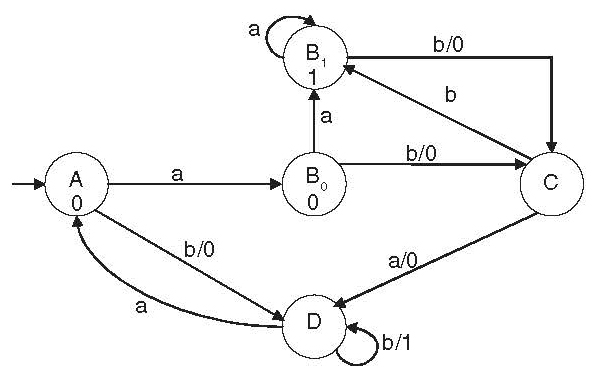
\includegraphics[width=5cm,height=3cm]{1.jpg}
\end{center}
For the state A, the incoming edges to this state are from $B_\{0\}$ to C with label $b/0$ and $B_\{1\}$ to C with label $b/0$. There is no difference in the outputs of the incoming edges to this state, and so in the constructing Moore machine the output for this state will be 0.\\

\begin{center}
\section{picture}
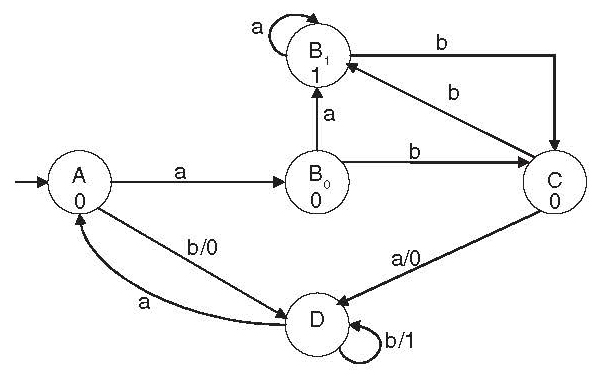
\includegraphics[width=5cm,height=3cm]{2.jpg}
\end{center}

For the state D, the incoming edges are A to D with label b/0, from C to D with label a/0, and from D to D with label b/1.\\
We get two different outputs for two incoming edges (D to D output 1, C to D output 0). So, the state D will be divided into two, namely, $D_\{0\}$ and $D_\{1\}$. The outgoing edges are duplicated for both the states generated from D. The modifi ed machine is
\begin{center}
\section{picture}
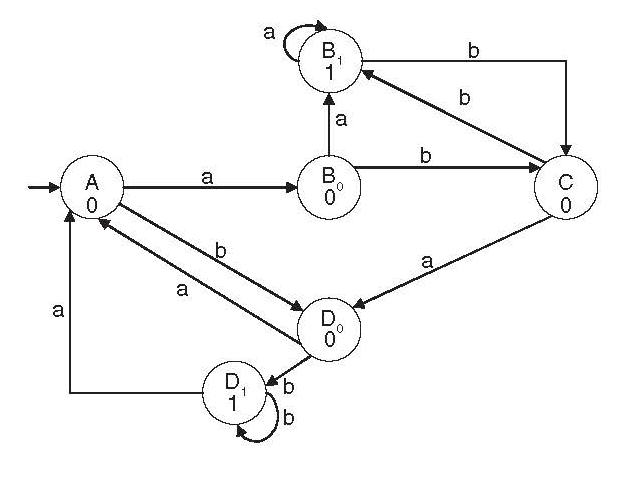
\includegraphics[width=5cm,height=3cm]{3.jpg}
\end{center}

\newpage
\begin{flushleft}
    \textbf{110}\hspace*{0.1cm} \textbf{$|$} \hspace*{0.1cm} \texttt{Introduction to Automata Theory, Formal Languages and Computation}
  \end{flushleft}

  \vspace*{0.5cm}
  \small{
\begin{multicols}{2}
21.Convert the following Mealy machine into an equivalent Moore machine. [UPTU 2004]\\
Solution: The state $q_0$ has two incoming edges: from $q_1$ with label a/0 and from $q_3$ with label $b/1$. As there is a difference in output, the state $q_0$ is divided into $q_00$ and $q_01$ with outputs 0 and 1, respectively. The states $q_1$ and $q_3$ have only one incoming edge each, and so there is no need of division. The state $q_2$ has three incoming edges; among those, two are of output '0' and another is of output '1'. Thus, it is divided into $q_20$ and $q_21$ with outputs 0 and 1, respectively.

\begin{center}
\section{picture}
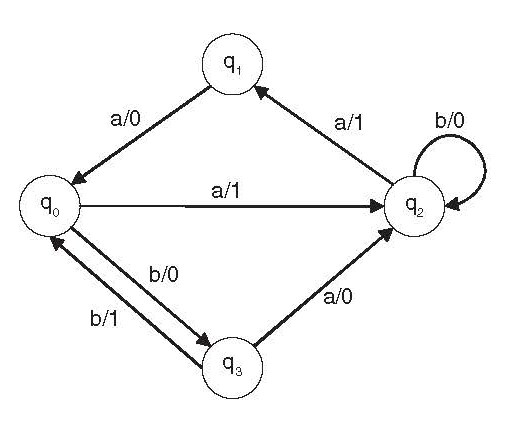
\includegraphics[width=5cm,height=3cm]{4.jpg}
\end{center}
\end{multicols}
}

From $q_1$ input with label 'a' ends on $q_00$, and from $q_3$ input with label 'b' ends on $q_01$. The outputs from old $q_1$ state are duplicated from $q_00$ and $q_01$.\\
The state $q_1$ and $q_3$ are not divided. $q_1$ gets output '1' and $q_3$ gets output '0'.
Dividing the state $q_0$ and placing $q_1$ and $q_3$, the intermediate machine becomes as follows\\
\begin{center}
\section{picture}
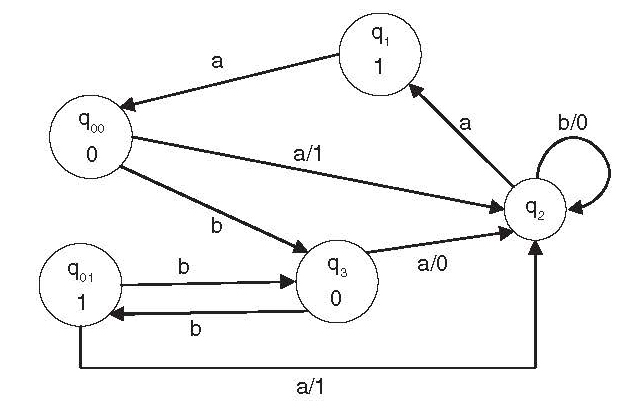
\includegraphics[width=5cm,height=3cm]{5.jpg}
\end{center}

The state $q_24$ is divided into $q_20$ and $q_21$. From $q_00$ and $q_01$ input with label 'a' ends on $q_21$. From $q_3$ input with label 'a' ends on $q_20$. There is a loop on $q_2$. That loop will be on $q_20$ with label 'b'. Another transition with label 'b' is drawn from $q_21$ to $q_20$. The final Moore machine is as follows\\
\begin{center}
\section{picture}
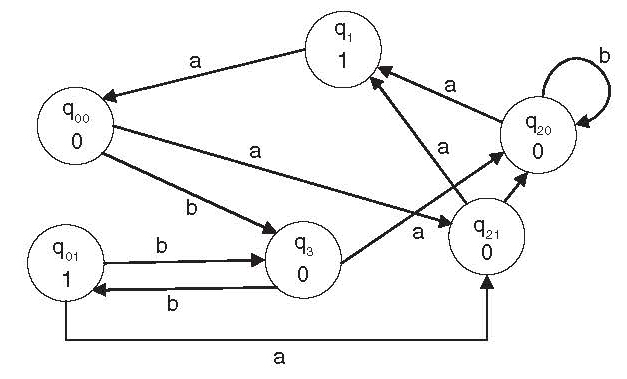
\includegraphics[width=5cm,height=3cm]{6.jpg}
\end{center}


22.Minimize the following finite automata.\\
\begin{center}
\begin{tabular}{rccc}
	\hline
	&&Next State\\
	\hline
	&Present State&I/P = a&I/P = b\\
	\hline
	$\rightarrow$&A&B&F\\
	&B&A&F\\
	&C&G&A\\
	&D&H&B\\
	&E&A&G\\
	&F&H&C\\
	&G&A&D\\
	&H&A&C\\
	\hline
\end{tabular}
\end{center}
Here F, G, and H are the final states.\\
Solution: In the finite automata, the states are $\{A, B, C, D, E, F, G, H\}$. Name this set as $S_0$.\\
$S_0: \{A, B, C, D, E, F, G, H\}$\\


All of the states are 0 equivalents.\\
In the finite automata, there are two types of states: final state and non-final states. So, divide the set of states into two parts, Q1 and Q2.\\
$Q_1 = \{F, G, H\} Q_2 = \{A, B, C, D, E\}$\\
$S_1: \{\{F, G, H\} \{A, B, C, D, E\}\}$\\
The states belonging to same subset are 1-equivalent because they are in the same set for string length 1. The states belonging to different subsets are 1-distinguishable.\\
The next states of F are H and C. The next states of G and H are A, D and A, C, respectively.\\
A, D and A, C belong to the same subset but H and C belong to a different subset. So, F, G, and H are divided into $\{F\}, \{G, H\}$.\\

For input 0, the next states of A, B, C, D, and E are B, A, G, H, and A, respectively. For input 1,the next states of A, B, C, D, and E are F, F, A, B, and G, respectively. So, the set $\{A, B, C, D, E\}$ is divided into $\{A, B, E\}$ and $\{C, D\}$.\\
             $S_2: \{\{F\} \{G, H\} \{A, B, E\} \{C, D\}\}$\\
By the same process, $\{A, B, E\}$ is divided into $\{A, B\}$, $\{E\}$.\\
$S_3: \{\{F\} \{G, H\} \{A, B\} \{E\} \{C, D\}\} = \{\{A, B\}, \{C, D\}, \{E\}, \{F\}, \{G, H\}\}$\\

The set is not dividable further. So, these are the states of minimized DFA. Let us rename the subsets as $q_0, q_1, q_2, q_3$, and $q_4$. The initial state was A, and so here the initial state is $\{A, B\}, i.e., q_0$. The final state was F, G, and H, and so here the fi nal states are $\{F\}, i.e., q_3$ and $\{G, H\}, i.e., q_4$. The tabular representation of minimized $DFA$ is
\\

\begin{center}

	\begin{tabular}{rccc}
		\hline
		&&Next State\\
		\hline
		&Present State&I/P = 0&I/P = 1\\
		\hline
		$\rightarrow$&$q_{0}$&$q_{0}$&$q_{0}$\\
		&$q_{0}$&$q_{0}$&$q_{0}$\\
		&$q_{0}$&$q_{0}$&$q_{0}$\\
		&$q_{0}$&$q_{0}$&$q_{0}$\\
		&$q_{0}$&$q_{0}$&$q_{0}$\\
		\hline
	\end{tabular}
\end{center}

23.Design a Mealy and Moore machine for detecting a sequence 1010 where overlapping sequences are also accepted. Convert the Moore machine that you have got into a Mealy machine. Are there any differences? How will you prove that the two Mealy machines are equivalent?\\
Solution: The Mealy machine is\\

\begin{center}
\section{picture}
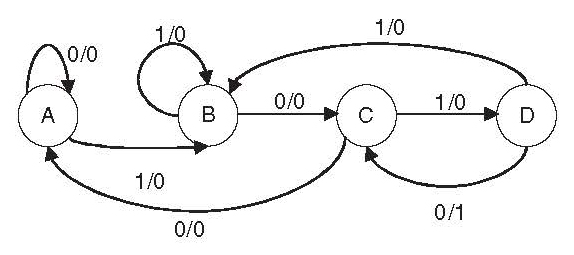
\includegraphics[width=5cm,height=3cm]{7.jpg}
\end{center}


The Moore machine is\\
\begin{center}
\section{picture}
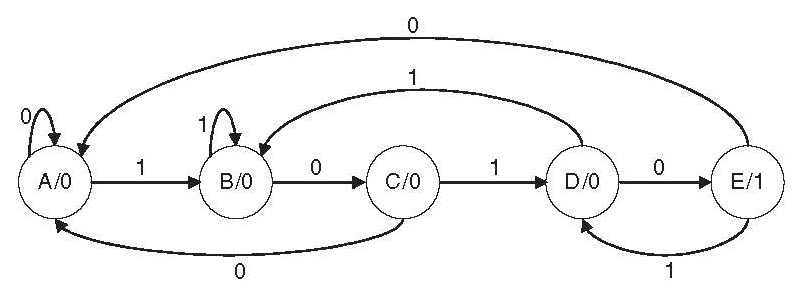
\includegraphics[width=5cm,height=3cm]{8.jpg}
\end{center}

The converted Mealy machine from the given Moore machine is (by using the transactional format)\\
\begin{center}
\section{picture}
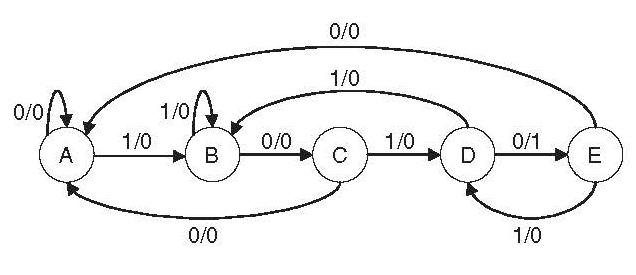
\includegraphics[width=5cm,height=3cm]{9.jpg}
\end{center}

\end{document}

